
%<<setup-child, include = FALSE>>=
%library(knitr)
%options(digits = 16)

%library(RCurl)
%library(XML)
%library(tm)
%library(NMF)
%library(microbenchmark)
%library(ggplot2)
%library(wordcloud)
%set_parent("../style/preamble.Rnw")
%@


\newcommand{\xdownarrow}[1]{%
  {\left\downarrow\vbox to #1{}\right.\kern-\nulldelimiterspace}
}

\newcommand{\grey}[1]{\textcolor{grey}{#1}}
\newcommand{\red}[1]{\textcolor{red}{#1}}


\input{../../2021/style/preamble4tex}
% dependencies: amsmath, amssymb, dsfont
% math spaces
\ifdefined\N
\renewcommand{\N}{\mathds{N}} % N, naturals
\else \newcommand{\N}{\mathds{N}} \fi
\newcommand{\Z}{\mathds{Z}} % Z, integers
\newcommand{\Q}{\mathds{Q}} % Q, rationals
\newcommand{\R}{\mathds{R}} % R, reals
\ifdefined\C
\renewcommand{\C}{\mathds{C}} % C, complex
\else \newcommand{\C}{\mathds{C}} \fi
\newcommand{\continuous}{\mathcal{C}} % C, space of continuous functions
\newcommand{\M}{\mathcal{M}} % machine numbers
\newcommand{\epsm}{\epsilon_m} % maximum error

% counting / finite sets
\newcommand{\setzo}{\{0, 1\}} % set 0, 1
\newcommand{\setmp}{\{-1, +1\}} % set -1, 1
\newcommand{\unitint}{[0, 1]} % unit interval

% basic math stuff
\newcommand{\xt}{\tilde x} % x tilde
\newcommand{\argmin}{\mathop{\mathrm{arg\,min}}} % argmin
\newcommand{\argmax}{\mathop{\mathrm{arg\,max}}} % argmax
\newcommand{\argminlim}{\argmin\limits} % argmin with limits
\newcommand{\argmaxlim}{\argmax\limits} % argmax with limits
\newcommand{\sign}{\operatorname{sign}} % sign, signum
\newcommand{\I}{\mathbb{I}} % I, indicator
\newcommand{\order}{\mathcal{O}} % O, order
\newcommand{\bigO}{\mathcal{O}} % Big-O Landau
\newcommand{\littleo}{{o}} % Little-o Landau
\newcommand{\pd}[2]{\frac{\partial{#1}}{\partial #2}} % partial derivative
\newcommand{\floorlr}[1]{\left\lfloor #1 \right\rfloor} % floor
\newcommand{\ceillr}[1]{\left\lceil #1 \right\rceil} % ceiling
\newcommand{\indep}{\perp \!\!\! \perp} % independence symbol

% sums and products
\newcommand{\sumin}{\sum\limits_{i=1}^n} % summation from i=1 to n
\newcommand{\sumim}{\sum\limits_{i=1}^m} % summation from i=1 to m
\newcommand{\sumjn}{\sum\limits_{j=1}^n} % summation from j=1 to p
\newcommand{\sumjp}{\sum\limits_{j=1}^p} % summation from j=1 to p
\newcommand{\sumik}{\sum\limits_{i=1}^k} % summation from i=1 to k
\newcommand{\sumkg}{\sum\limits_{k=1}^g} % summation from k=1 to g
\newcommand{\sumjg}{\sum\limits_{j=1}^g} % summation from j=1 to g
\newcommand{\summM}{\sum\limits_{m=1}^M} % summation from m=1 to M
\newcommand{\meanin}{\frac{1}{n} \sum\limits_{i=1}^n} % mean from i=1 to n
\newcommand{\meanim}{\frac{1}{m} \sum\limits_{i=1}^m} % mean from i=1 to n
\newcommand{\meankg}{\frac{1}{g} \sum\limits_{k=1}^g} % mean from k=1 to g
\newcommand{\meanmM}{\frac{1}{M} \sum\limits_{m=1}^M} % mean from m=1 to M
\newcommand{\prodin}{\prod\limits_{i=1}^n} % product from i=1 to n
\newcommand{\prodkg}{\prod\limits_{k=1}^g} % product from k=1 to g
\newcommand{\prodjp}{\prod\limits_{j=1}^p} % product from j=1 to p

% linear algebra
\newcommand{\one}{\bm{1}} % 1, unitvector
\newcommand{\zero}{\mathbf{0}} % 0-vector
\newcommand{\id}{\bm{I}} % I, identity
\newcommand{\diag}{\operatorname{diag}} % diag, diagonal
\newcommand{\trace}{\operatorname{tr}} % tr, trace
\newcommand{\spn}{\operatorname{span}} % span
\newcommand{\scp}[2]{\left\langle #1, #2 \right\rangle} % <.,.>, scalarproduct
\newcommand{\mat}[1]{\begin{pmatrix} #1 \end{pmatrix}} % short pmatrix command
\newcommand{\Amat}{\mathbf{A}} % matrix A
\newcommand{\Deltab}{\mathbf{\Delta}} % error term for vectors

% basic probability + stats
\renewcommand{\P}{\mathds{P}} % P, probability
\newcommand{\E}{\mathds{E}} % E, expectation
\newcommand{\var}{\mathsf{Var}} % Var, variance
\newcommand{\cov}{\mathsf{Cov}} % Cov, covariance
\newcommand{\corr}{\mathsf{Corr}} % Corr, correlation
\newcommand{\normal}{\mathcal{N}} % N of the normal distribution
\newcommand{\iid}{\overset{i.i.d}{\sim}} % dist with i.i.d superscript
\newcommand{\distas}[1]{\overset{#1}{\sim}} % ... is distributed as ...


\begin{document}


\lecturechapter{7}{Overdetermined Systems \& Regression Example}
\lecture{CIM1 Statistical Computing}


\begin{vbframe}{Overdetermined systems}

A system of linear equations $\bm{Ax} = \bm{b}$ with $\bm{A} \in \R^{m\times n}, m \ge n$ with more equations than unknowns, is called \textbf{overdetermined}.

\lz

In general such a system has no (exact) solution.

\lz

A (compromise) solution using \textbf{least squares} is the vector $\bm{x}$ which minimizes the squared sum of the \textbf{residual vector} $\bm{r} = \mathbf{b} - \mathbf{A}\boldsymbol{x}$:

$$
\bm{x} = \text{arg} \min \|\mathbf{b} - \mathbf{A}\boldsymbol{x}\|^2_2
$$

\end{vbframe}

\begin{vbframe}{Example: the regression model}

\textbf{Aim:} Solve $\bm{X}\boldsymbol{\beta} = \bm{y}$ with

\begin{itemize}
\item $\mathbf{X}$: $n \times (p + 1)$, Design matrix
\item $\mathbf{y}$: $n \times 1$, $n$ observations
% \item $\boldsymbol{\varepsilon}$: $n \times 1$ Fehlerterm
\item $\boldsymbol{\beta}$: $(p + 1) \times 1$, $p$ regressors plus intercept
\end{itemize}

Since the linear system is usually overdetermined (more observations than variables) and has no solution, we minimize the residual sum of squares:

$$
\min_\beta \|\mathbf{y} - \mathbf{X}\boldsymbol{\beta}\|^2_2 = (\mathbf{y} - \mathbf{X}\boldsymbol{\beta})^\top
  (\mathbf{y} - \mathbf{X}\boldsymbol{\beta})
$$

\lz

\textbf{Questions}: How can the problem be solved in a numerically stable way? Which algorithms are fast?


% Matrizenschreibweise:
% $$
% \mathbf{y} = \mathbf{X}\boldsymbol{\beta} + \boldsymbol{\varepsilon},
%  \qquad \E(\boldsymbol{\varepsilon}) = \mathbf{0},
% $$
% \begin{itemize}
% \item $\mathbf{y}$: $n \times 1$ Zufallsvektor, $n$ Beobachtungen
% \item $\boldsymbol{\varepsilon}$: $n \times 1$ Fehlerterm
% \item $\boldsymbol{\beta}$: $(p + 1) \times 1$, $p$ Regressoren plus Intercept,
% \item $\mathbf{X}$: $n \times (p + 1)$, Design-Matrix (für uns fest).
% \end{itemize}
% Minimale Anforderungen an den Fehlerterm:
% \begin{itemize}
% \item Klassisches Modell: $\cov(\boldsymbol{\varepsilon}) = \sigma^2 \mathbf{I}$.
% \item Allgemeines lineares Modell: $\cov(\boldsymbol{\varepsilon}) = \boldsymbol{\Sigma}$.
% \end{itemize}
% \end{vbframe}

% \begin{vbframe}{Least Squares Regression}
% \textbf{Ziel:} Minimieren der Quadratsumme der Fehler
% $$
% \min_\beta \|\mathbf{y} - \mathbf{X}\boldsymbol{\beta}\|^2_2 = (\mathbf{y} - \mathbf{X}\boldsymbol{\beta})^\top
%   (\mathbf{y} - \mathbf{X}\boldsymbol{\beta}).
% $$



% Falls $\mathbf{X}$ vollen Rang hat $\SpAr \hat{\boldsymbol{\beta}} =
%   (\mathbf{X}^\top\mathbf{X})^{-1}\mathbf{X}^\top\mathbf{y}$.\\

% \framebreak
%
% Residuenvektor
% $$
% \mathbf{e} = \mathbf{y} - \hat{\mathbf{y}} = \mathbf{y} - \mathbf{X}\hat{\boldsymbol{\beta}} =
%   \mathbf{y} - \mathbf{X}(\mathbf{X}^\top\mathbf{X})^{-1}\mathbf{X}^\top\mathbf{y} =
%   (\mathbf{I} - \mathbf{P})\mathbf{y},
% $$
% wobei  $\mathbf{P} = \mathbf{X}(\mathbf{X}^\top\mathbf{X})^{-1}\mathbf{X}^\top$ symmetrisch und
% idempotent. \\
% $\SpAr$ \textbf{Projektionsoperator}\\
% \medskip
% $\mathbf{P}$ \dots Projektion auf linearen Unterraum, der von $\mathbf{X}$ aufgespannt \\
% $\mathbf{I} - \mathbf{P}$ \dots Projektion auf Orthogonalraum\\
% \medskip
% Damit gilt für Residual Sum of Squares:
% $$
% RSS = Q(\hat{\boldsymbol{\beta}}) = \mathbf{y}^\top(\mathbf{I} - \mathbf{P})^\top(\mathbf{I} -
%   \mathbf{P})\mathbf{y} =  \mathbf{y}^\top(\mathbf{I} - \mathbf{P})\mathbf{y}
% $$

% \framebreak

% Anschaulich kann man sich klar machen, dass die Differenz $\|\mathbf{r}(\boldsymbol{\beta})\| = \|\mathbf{y} - \mathbf{X}\boldsymbol{\beta}\|_2$ dann minimal wird, wenn $\mathbf{y} - \mathbf{X}\boldsymbol{\beta}$ senkrecht auf dem Bildraum von $\text{Bild}(\mathbf{X}) = \{\mathbf{X} \boldsymbol{\beta} | \boldsymbol{\beta} \in \R^{p+1}\}$ steht.

% \begin{center}
% 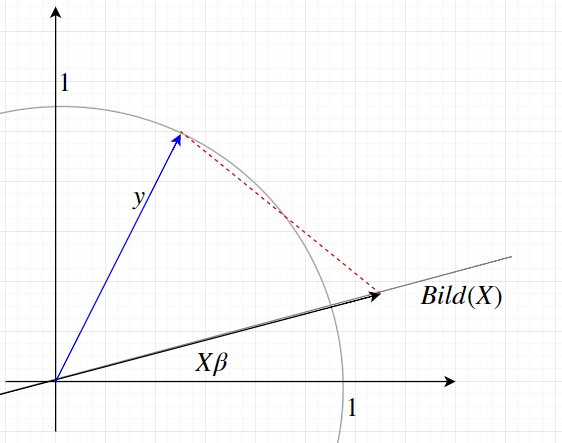
\includegraphics[width = 0.5\textwidth]{figure_man/ignore/regression.png} ~~ 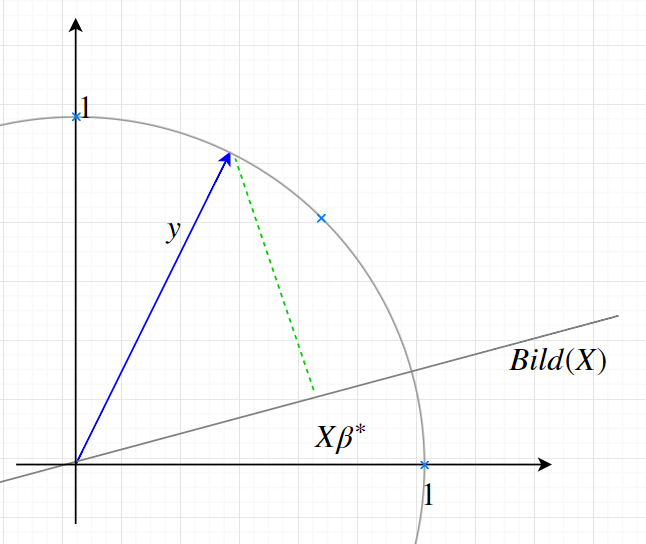
\includegraphics[width = 0.5\textwidth]{figure_man/ignore/regressionopt.png}
% \end{center}

% \end{vbframe}

% \begin{vbframe}{Kondition der Regression}

% Wir interessieren uns für die Berechnung des Parametervektors $\boldsymbol{\beta}$. Somit is $\boldsymbol{\beta}$ als Ergebnis und $\mathbf{y}$ bzw. $\mathbf{X}$ als Eingabe zu sehen.

% \lz

% Wie verändert sich das optimale $\boldsymbol{\beta}^*$ bei einer kleinen Störung von $\mathbf{y}$?


% \begin{center}
% 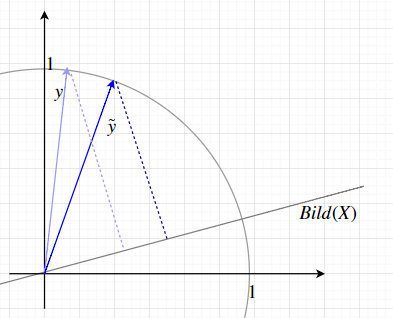
\includegraphics[width = 0.4\textwidth]{figure_man/ignore/regressionkonditionbad.png} ~~~ 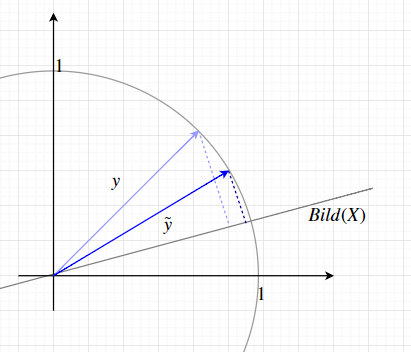
\includegraphics[width = 0.4\textwidth]{figure_man/ignore/regressionkonditiongood.png}
% \end{center}


% Notation:  $\tilde{\mathbf{y}} = \mathbf{y} + \Deltab \mathbf{y}$ eine kleine Abweichung von $\mathbf{y}$, $\boldsymbol{\beta}^*$ und $\tilde{\boldsymbol{\beta}}^*$ die jeweiligen Schätzer. \\

% \lz

% Dann gilt

% $$
% \frac{\|\boldsymbol{\beta}^* - \tilde{\boldsymbol{\beta}}^*\| }{\|\boldsymbol{\beta}^*\|}
%   \leq \frac{\kappa(\mathbf{X})}{\cos(\theta)} \frac{\|\Deltab \mathbf{y}\| }{\|{\mathbf{y}}\|}.
% $$

% Hierbei bezeichne

% \begin{itemize}
% \item $\kappa(\mathbf{X}):= \sqrt{\kappa(\mathbf{X}^T\mathbf{X})}$ die Kondition der $n \times (p + 1)$ Matrix $\mathbf{X}$,
% \item $\theta$ den Winkel zwischen $\mathbf{y}$ und dem Unterraum $\{\mathbf{X} \boldsymbol{\beta} | \boldsymbol{\beta} \in \R^{p+1}\}$.
% \end{itemize}

% Die Kondition des linearen Ausgleichsproblems bzgl. Störungen in $\mathbf{y}$ kann also abgeschätzt werden durch $\frac{\kappa(\mathbf{X})}{\cos(\theta)}$.

% \framebreak

% Bezüglich Störungen der Matrix $\tilde{\mathbf{X}} = \mathbf{X} + \Deltab \mathbf{X}$ ergibt sich ein etwas komplizierteres Resultat

% $$
% \frac{\|\boldsymbol{\beta}^* - \tilde{\boldsymbol{\beta}}^*\| }{\|\boldsymbol{\beta}^*\|}
%   \leq \biggl(\kappa(\mathbf{X}) + \kappa(\mathbf{X})^2\tan \theta\biggr) \frac{\|\Deltab \mathbf{X}\| }{\|{\mathbf{X}}\|}.
% $$

% Die Konditionszahl bzgl. Störungen in $\mathbf{X}$ lautet also

% $$
% \kappa(\mathbf{X}) + \kappa(\mathbf{X})^2\tan \theta.
% $$

% \vfill

% \begin{footnotesize}
% Eine Herleitung für obige Resultate ist hier zu finden:
% \emph{Deuflhard, Numerische Mathematik I, 2001, Kapitel 3}
% \end{footnotesize}

% \framebreak

% \begin{itemize}
% \item In beiden Formeln sieht man: Die Kondition des linearen Ausgleichsproblems hängt also nicht nur von der Kondition der Matrix $\mathbf{X}$, sondern auch von der Größe des Winkels $\theta$ und damit der Größe des Residuums $\mathbf{r} := \mathbf{y} - \mathbf{X} \boldsymbol{\beta}^*$ ab.
% \item Für kleine Residuen, also $\cos\theta \approx 1$ und $\tan \theta \approx 0$, verhält sich das lineare Ausgleichsproblem konditionell wie ein lineares Gleichungssystem.
% \item Für große Residuen, also $\cos \theta \ll 1$ und $\tan\theta \gg 1$, verhält sich das lineare Ausgleichsproblem konditionell wesentlich anders als lineare Gleichungssysteme.
% \end{itemize}

% wobei $\kappa^* := \sqrt{\kappa(\mathbf{X}^\top\mathbf{X})}$\\
% \medskip
% Nur Störungen von $\mathbf{y}$, die tatsächlich Einfluss auf die geschätzte Lösung haben,
% wirken sich auf geschätzte Koeffizienten aus $\SpAr$ sinnvolles Resultat für Regressionsdiagnostik.

\end{vbframe}

\begin{vbframe}{Condition of normal equations}

The solution of the optimization problem is (mathematically) equivalent to the solution of the \textbf{normal equation}
$$
\mathbf{X}^\top\mathbf{X}\boldsymbol{\beta} = \mathbf{X}^\top\mathbf{y}
$$

(Derivation: differentiate with respect to $\boldsymbol{\beta}$ and set to $0$).

If the matrix $\mathbf{X}$ has full column rank, then the matrix $\mathbf{X}^\top \mathbf{X}$ is symmetric positive-definite and the following holds

\begin{eqnarray*}
\kappa(\mathbf{X}^T\mathbf{X}) &=& \kappa(\mathbf{X})^2
\end{eqnarray*}

using the spectral norm.

\lz

Consequently, the error amplification is $\kappa(\mathbf{X})^2$ when using normal equations.

\framebreak

\textbf{Note:}
\begin{itemize}
\item Mathematically speaking, the solution of the normal equations is equivalent to the minimization of the residual sum of squares
\item However, from a numerical point of view a distinction must be made between the two of them
\item A solution using the normal equations requires the calculation of $\mathbf{X}^\top \mathbf{X}$, an error in $\mathbf{X}$ is therefore amplified
% \item For small residuals, the condition is described by $\approx \kappa(\mathbf{X})$, so the condition $\kappa(\mathbf{X}^T\mathbf{X}) = \kappa(\mathbf{X})^2$ (!!) for solution over normal equations
% \item The solution of linear equilibrium problems via normal equations can (if at all) be recommended only for large residuals
\item Better: Find an efficient method that operates directly on $\mathbf{X}$
\end{itemize}




% \framebreak
%
% Resultat für Störungen in $\mathbf{X}$ um einiges komplizierter.\\
% \medskip
% Sei $\mathbf{E}$ Störung von $\mathbf{X}$ und  $\hat{\boldsymbol{\beta}}^*$  zugehörige Lösung
% $$
% \frac{\|\hat{\boldsymbol{\beta}} - \hat{\boldsymbol{\beta}}^*\| }{\|\hat{\boldsymbol{\beta}}\|}
%   \leq 2\kappa^* \frac{\|\mathbf{P}\mathbf{E}\| }{\|\mathbf{X}\|}
% + 4 (\kappa^*)^2  \frac{\|\hat{\mathbf{e}}\|}{\|\hat{\mathbf{y}}\|}
%   \frac{\|(\mathbf{I} - \mathbf{P})\mathbf{E}\| }{\|\mathbf{X}\|}
% + 8 (\kappa^*)^3   \frac{\|(\mathbf{I} - \mathbf{P})\mathbf{E}\|^2 }{\|\mathbf{X}\|^2}
% $$
% Bemerkungen:
% \begin{itemize}
% \item Falls Störung $\mathbf{E}$ hinreichend klein, dritter Term vernachlässigbar.
% \item  Falls $\|\hat{\mathbf{e}}\| \ll \|\hat{\mathbf{y}}\|$, dann zweiter Term vernachlässigbar. \\
% Falls Modell nicht so gut passt, dann Kondition $(\kappa^*)^2$.
% \item Typischerweise $\|\mathbf{PE}\| \approx \|(\mathbf{I} - \mathbf{P})\mathbf{E}\|$.
% \item Beachte: Große Konditionszahl geht typischerweise einher mit großen Konfidenzintervallen, weil
% $\cov(\hat{\boldsymbol{\beta}}) = \sigma^2 (\mathbf{X}^\top\mathbf{X})^{-1}$.
% \end{itemize}
\end{vbframe}



% \begin{vbframe}{Gauß-Markov-Theorem}
% Klassisches Modell: $\mathbf{y} = \mathbf{X}\boldsymbol{\beta} + \boldsymbol{\varepsilon}, \quad
%   \E(\boldsymbol{\varepsilon}) = \mathbf{0}, \quad \cov(\boldsymbol{\varepsilon}) = \sigma^2 \mathbf{I}$.\\
% \medskip
% Dann gilt:
% \begin{itemize}
% \item $\E(\hat{\boldsymbol{\beta}}) = \boldsymbol{\beta}$ unverzerrter Schätzer,
% \item $\cov(\hat{\boldsymbol{\beta}}) = \sigma^2(\mathbf{X}^\top\mathbf{X})^{-1}$,
% \item $\hat{\boldsymbol{\beta}}$ ist BLUE (best linear unbiased),
% \item $\hat{\sigma}^2 = RSS/(n-p-1)$ ist unverzerrter Schätzer der Varianz.
% \end{itemize}
% Berechnung von $(\mathbf{X}^\top\mathbf{X})^{-1}$ nicht notwendig, um $\hat{\boldsymbol{\beta}}$
% zu schätzen.\\
% \medskip
% Allerdings z.B.\ notwendig für Konfidenzintervalle von $\beta_i$.
% \end{vbframe}

\begin{vbframe}{Solution of the normal equations}

Model $\mathbf{y} = \mathbf{X}\boldsymbol{\beta} + \boldsymbol{\varepsilon}$\\
\medskip
Normal equations: $ \qquad \mathbf{X}^\top\mathbf{X}\boldsymbol{\beta} = \mathbf{X}^\top\mathbf{y}$\\
\medskip
If $\mathbf{X}$ is of full rank then $\mathbf{X}^\top\mathbf{X}$ is positive-definite and the Cholesky decomposition applicable.
% \begin{itemize}
% \item Speichereffizient,
% \item Nachteil 1: Berechnung von $\mathbf{X}^\top\mathbf{X}$ explizit notwendig,
% \item Nachteil 2: Konditionszahl des Verfahrens $\kappa(\mathbf{X}^\top\mathbf{X})$, \\ während an sich nur $\sqrt{\kappa(\mathbf{X}^\top\mathbf{X})}$ für Problem der linearen Regression.
% \end{itemize}

\begin{enumerate}
\item Calculate $\mathbf{X}^\top\mathbf{X}$ and $\mathbf{X}^\top\mathbf{y}$,
\item Cholesky decomposition $\mathbf{X}^\top\mathbf{X} = \mathbf{LL}^\top$,
\item Solve $\mathbf{Lw} = \mathbf{X}^\top\mathbf{y}$ for $\mathbf{w}$,
\item Calculate $RSS = \mathbf{y}^\top\mathbf{y} - \mathbf{w}^\top\mathbf{w}$,
\item Solve $\mathbf{L}^\top\boldsymbol{\beta} = \mathbf{w}$ for $\boldsymbol{\beta} = \hat{\boldsymbol{\beta}}$,
\item $(\mathbf{X}^\top\mathbf{X})^{-1} = \mathbf{L}^{-\top}\mathbf{L}^{-1}$.
\end{enumerate}

\framebreak
\footnotesize
\begin{verbbox}
X = matrix(c(rep(1, 6), c(1.01, 1.01)), ncol = 2)
X
## [,1] [,2]
## [1,] 1 1.00
## [2,] 1 1.00
## [3,] 1 1.01
## [4,] 1 1.01
XX = t(X) %*% X
XX
## [,1] [,2]
## [1,] 4.00 4.020000000000000
## [2,] 4.02 4.040200000000000
\end{verbbox}
\col

\framebreak
\begin{verbbox}
XX2 = round(XX, 3)
XX2
## [,1] [,2]
## [1,] 4.00 4.02
## [2,] 4.02 4.04
\end{verbbox}
\col
\vspace{0.2cm}
\begin{verbbox}
cholesky(XX)
## [,1] [,2]
## [1,] 2.00 0.00000000000000000
## [2,] 2.01 0.01000000000007716
\end{verbbox}
\col
\vspace{0.2cm}
\begin{verbbox}
cholesky(XX2)
## [,1] [,2]
## [1,] 2.00 0
## [2,] 2.01 NaN
\end{verbbox}
\col

\normalsize
%<<include = FALSE>>=
%cholesky = function(a) {
%  n = nrow(a)
%  l = matrix(0, nrow = n, ncol = n)
%  for (j in 1:n) {
%    l[j, j] = (a[j, j] - sum(l[j, 1:(j - 1)]^2))^0.5
%    if (j < n) {
%      for (i in (j + 1):n) {
%        l[i, j] = (a[i, j] -
%          sum(l[i, 1:(j - 1)] * l[j, 1:(j - 1)])) / l[j, j]
%      }
%    }
%  }
%  return(l)
%}
%@


%<<>>=
%X = matrix(c(rep(1, 6), c(1.01, 1.01)), ncol = 2)
%X
%XX = t(X) %*% X
%XX
%@

%<<>>=
%XX2 = round(XX, 3)
%XX2
%@
%\vspace*{-0.3cm}
%<<>>=
%cholesky(XX)
%cholesky(XX2)
%@
\vspace{0.4cm}
$\Rightarrow$ Number of decimal digits matters, matrix no longer positive-definite!

\framebreak

In general a solution using  normal equations is to be avoided

$$
\mathbf{X}^\top\mathbf{X}\boldsymbol{\beta} = \mathbf{X}^\top\mathbf{y}
$$

since:

\begin{itemize}
\item \textbf{High computational effort}: First calculation of $\bm{X}^\top\bm{X}$, then matrix decomposition of $\bm{X}^\top\bm{X}$, then forward and back substitution
\item \textbf{Numeric instability}: In all these individual steps there is a risk that errors will be amplified.\\
\medskip
A further problem occurs if we want to solve the normal equations in case of \textbf{collinearity} in the design matrix $\mathbf{X}$.
The reason for this is the singularity of the product of $\mathbf{X}^\top\mathbf{X}$ which results from collinearity.
\end{itemize}

It is often more suitable to operate directly on $\mathbf{X}$ by using QR decomposition $\mathbf{X} = \mathbf{QR}$:

$$
\mathbf{X}^\top\mathbf{X} = (\mathbf{QR})^\top(\mathbf{QR}) = \mathbf{R}^\top\mathbf{Q}^\top\mathbf{QR} =
\mathbf{R}^\top\mathbf{R}
$$
The normal equations can then be written as
$$
\mathbf{R}^\top\mathbf{R}\boldsymbol{\beta} = \mathbf{R}^\top\mathbf{Q}\top\mathbf{y}
$$
and since $\mathbf{R}^\top$ is nonsingular it follows
$$
\mathbf{R}\boldsymbol{\beta} = \mathbf{Q}^\top\mathbf{y} % \quad \Rightarrow \quad \boldsymbol{\beta} =
  % \mathbf{R}^{-1}\mathbf{Q}^\top\mathbf{y} = (\mathbf{X}^\top\mathbf{X})^{-1}\mathbf{X}^\top\mathbf{y}.
$$

Since $\textbf{R}$ is an upper triangular matrix, the equation system (after multiplying $\bm{Q}^\top \bm{y}$) can be solved using back substitution in $\order(n^2)$.

\framebreak

The steps to solve a linear regression problem using QR decomposition are therefore as follows:

\begin{enumerate}
\item Calculate the QR decomposition $\mathbf{X} = \mathbf{Q}\mathbf{R}$,
\item Calculate $\bm{z} = \bm{Q}^\top \bm{y}$,
\item Solve the equation system $\bm{R}\boldsymbol{\beta} = \bm{z}$ using back substitution.
\end{enumerate}

\framebreak

\textbf{Advantage of QR decomposition:} As already stated, the solution when using QR decomposition can be written as
$$
\mathbf{R}\boldsymbol{\beta} = \mathbf{Q}^\top\mathbf{y}
$$

\begin{itemize}
\item $\mathbf{X}$ (and not $\bm{X}^\top\bm{X}$) is decomposed directly.
\item $\mathbf{X}^\top\mathbf{X}$ does not have to be calculated (thus avoiding numerical instability from collinearity).\\
\item If a stable algorithm is used to calculate the QR decomposition (e.g. Householder), the method is stable.
\item Extreme runtime advantages if a regression is to be performed for constant design matrix $\bm{X}$, but different $\bm{y}$.
\end{itemize}

\textbf{Note:} For linear models \texttt{lm()} in \texttt{R} the QR decomposition is applied when calculating $\boldsymbol{\beta}$.

\end{vbframe}

\begin{vbframe}{QR decomposition and ridge regression}

In order to avoid a high variance, large parameters are often penalized by a penalty term. We minimize a penalized version of the residual sum of squares

$$
\min_\beta \|\bm{y} - \bm{X\beta}\|_2^2 + \lambda \|\bm{\beta}\|_2^2
$$

with regularization parameter $\lambda > 0$. If the $L_2$ norm is selected for the penalty, the procedure is known as \textbf{ridge regression}.

\lz

We obtain a general version of the normal equations by setting the first derivative to $0$ 

$$
\left(\mathbf{X}^\top\mathbf{X} + \lambda I \right)\boldsymbol{\beta} = \mathbf{X}^\top\mathbf{y}
$$

\framebreak

With $\bm{A} \coloneqq \bigl( \begin{smallmatrix} \bm{X} \\ \sqrt{\lambda} \bm{I} \end{smallmatrix} \bigr) \in \mathbb{R}^{n+p,p} $  the normal equations for ridge regression can be rewritten as
\begin{eqnarray*}
\left(\mathbf{X}^\top\mathbf{X} + \lambda I \right)\boldsymbol{\beta} &=& \mathbf{X}^\top\mathbf{y} \\
\mathbf{A}^\top\mathbf{A}\boldsymbol{\beta} &=& \mathbf{A}^\top\begin{pmatrix} \mathbf{y} \\ \mathbf{0} \end{pmatrix}
\end{eqnarray*}
We use the QR decomposition of $ \bm{A} = \bm{Q}_\lambda\bm{R}_\lambda $ depending on $\lambda$:
\begin{eqnarray*}
\mathbf{A}^\top\mathbf{A}\boldsymbol{\beta} &=& \mathbf{A}^\top \begin{pmatrix} \mathbf{y} \\ \mathbf{0} \end{pmatrix} \\
\mathbf{R}_\lambda^\top \mathbf{Q}_\lambda^\top \mathbf{Q}_\lambda\mathbf{R}_\lambda\boldsymbol{\beta} &=& \mathbf{R}_\lambda^\top\mathbf{Q}_\lambda^\top \begin{pmatrix} \mathbf{y} \\ \mathbf{0} \end{pmatrix} \\
\mathbf{R}_\lambda^\top\mathbf{R}_\lambda\boldsymbol{\beta} &=& \mathbf{R}_\lambda^\top\mathbf{Q}_\lambda^\top \begin{pmatrix} \mathbf{y} \\ \mathbf{0} \end{pmatrix} 
\end{eqnarray*}

\begin{itemize}
\item If $\bm{R}_\lambda$ is singular, we have to solve two LES in echelon form
\item If $\bm{R}_\lambda$ is nonsingular and thus invertible, the equation simplifies to one linear system in echelon form
\end{itemize}

%\framebreak
\lz
The regularization parameter $\lambda$ is a hyperparameter that must be selected by the user. Often the linear system has to be solved several times for different $\lambda$ to find a sensible degree of regularization.
  
\medskip

In such situations the QR decomposition
\vspace*{-0.2cm}
\begin{eqnarray*}
\mathbf{R}_\lambda^\top\mathbf{R}_\lambda\boldsymbol{\beta} &=& \mathbf{R}_\lambda^\top\mathbf{Q}_\lambda^\top \begin{pmatrix} \mathbf{y} \\ \mathbf{0} \end{pmatrix} 
\end{eqnarray*}

has to be calculated anew for each $\lambda$. The QR decomposition of the matrix $\bm{A}$ is calculated in $\order(n^3)$. Forward and back substitution are operations of $\order(n^2)$, so in total the runtime is given by $\order(n^3)$.

% The calculation of the matrix $\boldsymbol{R_\lambda}$ and the solution of the equation system by back substitution (since $\boldsymbol{R_\lambda}$ upper triangle matrix) is $\order(n^2)$.


\end{vbframe}

\begin{vbframe}{Comparison of methods for regression}

\begin{footnotesize}
\begin{table}
\centering
\begin{tabular}{c|c|c|c}
Method                    & Runtime         & General Numerical Stability & Stability in Collinearity\\
\hline
Naive approach            &   - -           & no                        & no \\
LU                        &   + +           & yes, with pivotisation    & no \\
QR (Householder)          &   -             & yes                       & yes\\

\end{tabular}
\end{table}
\end{footnotesize}

\lz

$\Rightarrow$ \textbf{Note:} QR decomposition is not the fastest method regarding runtime, but it is always numerically stable in a regression context.

\framebreak

\lz


\begin{center}
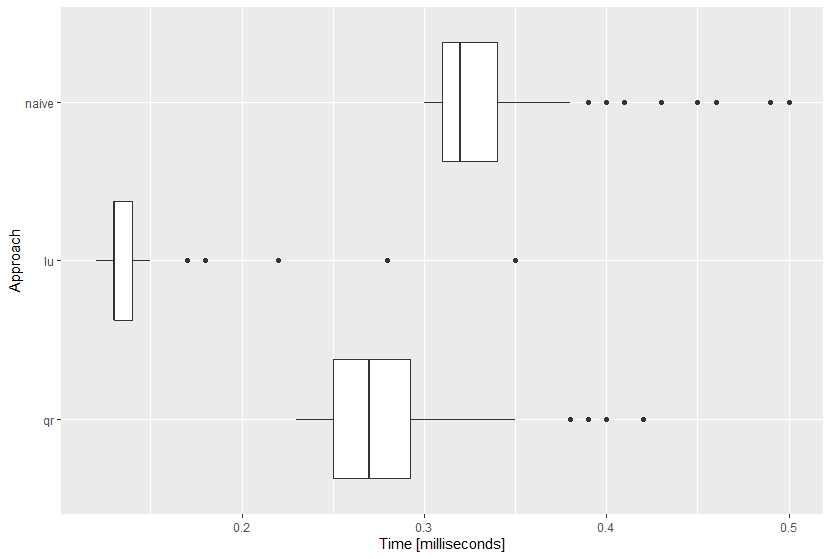
\includegraphics[width = 0.9\textwidth]{figure_man/method_comparison.png} 
\end{center}

% <<echo = F>>=
% set.seed(1)
% X = matrix(rnorm(500*20), 500, 20)
% y = rnorm(500)
% modelBenchmark <- microbenchmark(
%   qr = qr.coef(qr(X), y),
%   lu = solve(crossprod(X),crossprod(X, y)),
%   naive = solve(t(X) %*% X) %*% t(X) %*% y
% )
% @
% 
% 
% <<echo = F, out.width='90%', fig.align='center'>>=
% p = ggplot(modelBenchmark, aes(x = expr, y = round(time/1000000,digits = 2)))+
%   geom_boxplot() +
%   coord_flip() +
%   labs(x = "Approach",y = "Time [milliseconds]")
% p
% @

\end{vbframe}

% \textbf{Problem in der Praxis:}\\
% An sich sehr einfache Berechnung von $\mathbf{R}\boldsymbol{\beta} = \mathbf{Q}^\top\mathbf{y}$.\\
% \medskip
% ABER: $\mathbf{Q}$ nach obigem Algorithmus aus numerischen Gründen oft
% nicht wirklich orthogonal.\\
% \medskip
% {\bf Lösung:} Modifizierte Gram-Schmidt-Ortogonalisierung (MGS), \\
% für Details siehe Monahan bzw.\ Carl D.\ Meyer \emph{Matrix Analysis and Applied Linear Algebra}.
%
% \framebreak
%
% Zwei weitere Methoden für QR-Zerlegung\\
% \medskip
% {\bf Householder Matrizen:}\\
% \medskip
% Für Vektor $\mathbf{u}$ ist Matrix $\mathbf{U} = \mathbf{I} - d\mathbf{uu}^\top$ orthogonal,
% falls $d = 2/ \mathbf{u}^\top\mathbf{u}$.
% Wähle $\mathbf{u} = \mathbf{x} + s\mathbf{e}_1$ mit $s = \mathbf{x}^\top\mathbf{x}$
% $\SpAr \mathbf{Ux} = - s\mathbf{e}_1$.\\
% \medskip
% Sukzessive Elimination von Spaltenelementen liefert QR-Zerlegung.\\
% \medskip
% {\bf Givens Matrizen:}\\
% \medskip
% Ähnliches Prinzip zu Householder, aber orthogonale Transformationen, die jeweils
% ein Element eines Spaltenvektors eliminieren, und nur einen zweiten Vektor verändern.\\
% \medskip
% Für Details siehe Monahan bzw.\ Carl D.\ Meyer \emph{Matrix Analysis and Applied Linear Algebra}.


\endlecture
\end{document}







